\documentclass[a4paper]{article}

\usepackage[a4paper]{geometry}
\geometry{verbose,tmargin=2.5cm,bmargin=2.5cm,lmargin=2.5cm,rmargin=2.5cm}

\setlength{\parskip}{\smallskipamount}
\setlength{\parindent}{0pt}

\usepackage{fontspec}
\setmonofont{FreeMono}

\usepackage{hyperref}
\usepackage{url}
\usepackage{xcolor}

\usepackage{amsmath}
\usepackage{amssymb}

\usepackage{graphicx}
\usepackage{float}

\usepackage{minted}
\newminted{julia}{breaklines,fontsize=\small}
\newminted{bash}{breaklines,fontsize=\small}
\newminted{text}{breaklines,fontsize=\small}

\newcommand{\txtinline}[1]{\mintinline{text}{#1}}
\newcommand{\jlinline}[1]{\mintinline{julia}{#1}}

\newmintedfile[juliafile]{julia}{breaklines,fontsize=\small}

\begin{document}

\title{Implementing Density Functional Theory using Finite Difference Method}
\author{Fadjar Fathurrahman}
\date{}
\maketitle


\section{Overview}

Kohn-Sham equations:
\begin{equation}
\hat{H}_{\mathrm{KS}}\,\psi_{i}(\mathbf{r}) = \epsilon_{i}\,\psi_{i}(\mathbf{r})
\end{equation}


\section{Schroedinger equation in 1d}

We are interested in finding bound states solution to 1d time-independent Schroedinger equation:
\begin{equation}
\left[ -\frac{1}{2}\frac{\mathrm{d}^2}{\mathrm{d}x^2} + V(x) \right] \psi(x) = E\, \psi(x)
\label{eq:Sch_1d_eq}
\end{equation}
%
with the boundary conditions:
%
\begin{equation}
\lim_{x \rightarrow \pm \infty} \psi(x) = 0
\label{eq:BC_isolated}
\end{equation}
%
First we need to define a spatial domain $\left[x_{\mathrm{min}}, x_{\mathrm{max}}\right]$
where $x_{\mathrm{min}}, x_{\mathrm{max}}$ chosen
such that the boundary condition \ref{eq:BC_isolated} is approximately satisfied.
The next step is to divide the spatial domain $x$ using equally-spaced grid points
which we will denote as $\{x_{1},x_{2},\ldots,x_{N}\}$ where $N$ is number
of grid points. Various spatial quantities such as wave function and potential will be discretized
on these grid points.
The grid points $x_{i}$, $i = 1, 2, \ldots$ are chosen as:
\begin{equation}
x_{i} = x_{\mathrm{min}} + (i-1)h
\end{equation}
where $h$ is the spacing between the grid points:
\begin{equation}
h = \frac{ x_{\mathrm{max}} - x_{\mathrm{min}} }{N-1}
\end{equation}

The following code can be used to initialize the grid points:
\begin{juliacode}
function init_FD1d_grid( x_min::Float64, x_max::Float64, N::Int64 )
    L = x_max - x_min
    h = L/(N-1) # spacing
    x = zeros(Float64,N) # the grid points
    for i = 1:N
        x[i] = x_min + (i-1)*h
    end
    return x, h
end
\end{juliacode}


Approximating second derivative

Our next task is to find an approximation to the second derivative operator
present in the Equation \eqref{eq:Sch_1d_eq}.
One simple approximation that we can use is the 3-point (central) finite difference:
\begin{equation}
\frac{\mathrm{d}^2}{\mathrm{d}x^2} \psi_{i} =
\frac{\psi_{i+1} - 2\psi_{i} + \psi_{i-1}}{h^2}
\end{equation}
where we have the following notation have been used: $\psi_{i} = \psi(x_{i})$.
%
By taking $\{ \psi_{i} \}$ as a column vector, the second derivative operation
can be expressed as matrix multiplication:
\begin{equation}
\vec{\psi''} = \mathbb{D}^{(2)} \vec{\psi}
\end{equation}
%%
where $\mathbb{D}^{(2)}$ is the second derivative matrix operator:
\begin{equation}
\mathbb{D}^{(2)} = \frac{1}{h^2}
\begin{bmatrix}
-2  &  1  &  0  &  0  & 0 & \cdots & 0 \\
 1  & -2  &  1  &  0  & 0 & \cdots & 0 \\
 0  &  1  & -2  &  1  & 0 & \cdots & 0 \\
 \vdots  &  \ddots  &  \ddots  & \ddots  & \ddots  & \ddots & \vdots \\
 0 & \cdots & 0 & 1 & -2 & 1 & 0 \\
 0  &  \cdots  & \cdots & 0  & 1  & -2  & 1 \\
 0  &  \cdots  & \cdots & \cdots & 0  &  1  & -2 \\
\end{bmatrix}
\label{eq:1d_D2_matmul}
\end{equation}

An example implementation can be found in the following function.
\begin{juliacode}
function build_D2_matrix_3pt( N::Int64, h::Float64 )
    mat = zeros(Float64,N,N)
    for i = 1:N-1
        mat[i,i] = -2.0
        mat[i,i+1] = 1.0
        mat[i+1,i] = mat[i,i+1]
    end
    mat[N,N] = -2.0
    return mat/h^2
end
\end{juliacode}


Before use this function to solve Schroedinger equation we will to test the operation
in Equation \eqref{eq:1d_D2_matmul} for a simple function which second derivative
can be calculated analytically.
\begin{equation}
\psi(x) = \mathrm{e}^{-\alpha x^2}
\end{equation}
%
which second derivative can be calculated as
%
\begin{equation}
\psi''(x) = \left( -2 \alpha + 4\alpha^2 x^2 \right) \mathrm{e}^{-\alpha x^2}
\end{equation}
%
They are implemented in the following code
\begin{juliacode}
function my_gaussian(x; α=1.0)
    return exp(-α*x^2)
end

function d2_my_gaussian(x; α=1.0)
    return (-2*α + 4*α^2 * x^2) * exp(-α*x^2)
end
\end{juliacode}

\begin{figure}[H]
{\center
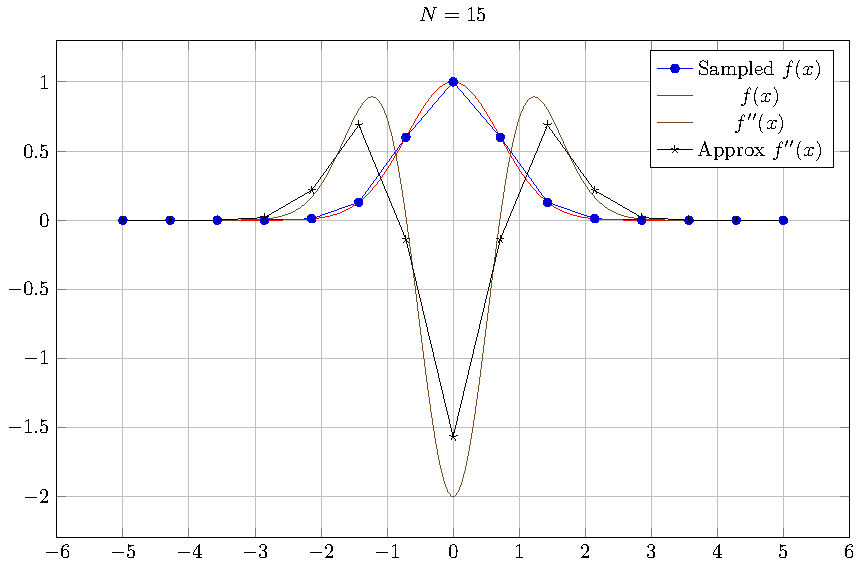
\includegraphics[scale=0.75]{../codes/IMG_gaussian_15.pdf}
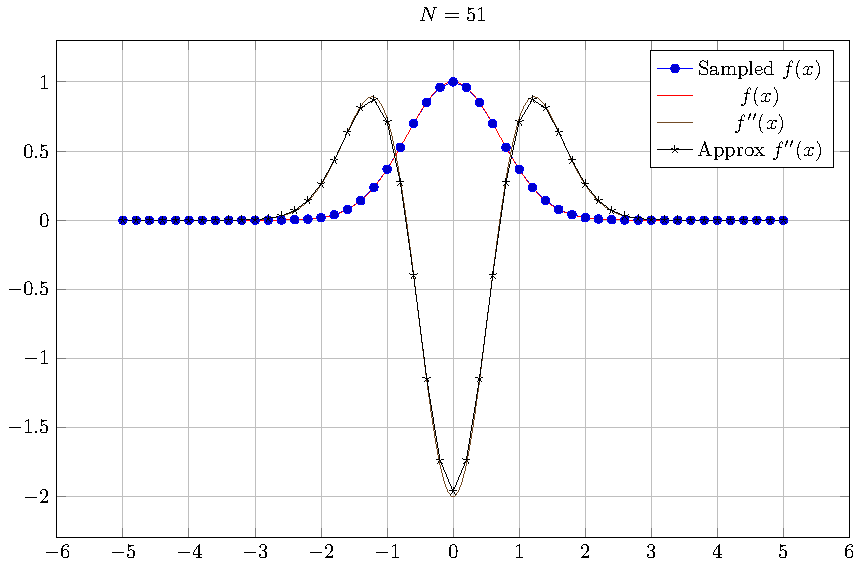
\includegraphics[scale=0.75]{../codes/IMG_gaussian_51.pdf}
\par}
\caption{Finite difference approximation to a Gaussian function and its second derivative}
\end{figure}


Harmonic potential

We will start with a simple potential with known exact solution, namely the harmonic potential:
\begin{equation}
V(x) = \frac{1}{2}\omega^2 x^2
\end{equation}

The Hamiltonian in finite difference representation:
\begin{equation}
\mathbb{H} = -\frac{1}{2}\mathbb{D}^{(2)} + \mathbb{V}
\end{equation}
where $\mathbb{V}$ is a diagonal matrix whose elements are:
\begin{equation}
\mathbb{V}_{ij} = V(x_{i})\delta_{ij}
\end{equation}


Code to solve harmonic oscillator:

\juliafile{../codes/main_harmonic_01.jl}

Compare with analytical solution.

Plot of eigenfunctions:

\begin{figure}[H]
{\center
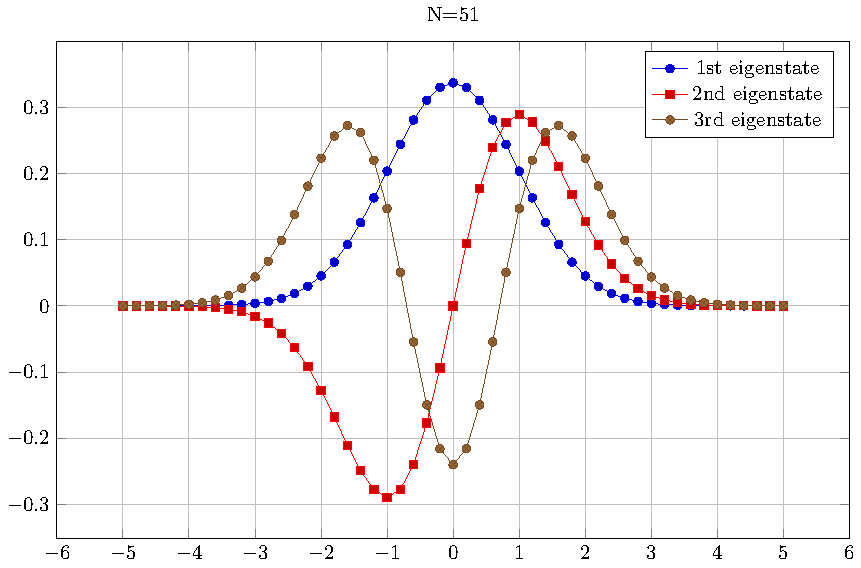
\includegraphics[scale=0.75]{../codes/IMG_main_harmonic_01_51.pdf}
\par}
\caption{Eigenstates of harmonic oscillator}
\end{figure}


\section{Higher order finite difference}

To obtain higher accuracy

Implementing higher order finite difference.



\appendix

\section{Alternative solutions}

\begin{juliacode}
function my_func()
    println("OK ...")
end
\end{juliacode}


\end{document}